\documentclass[letterpaper,12pt,fleqn]{article}
\usepackage{matharticle}
\usepackage{mathtools}
\pagestyle{plain}
\begin{document}

\begin{center}
\Large Math-08 Homework \#8
\end{center}

\vspace{0.5in}

\underline{Reading}

\begin{itemize}
\item Text book section 1.2,1.6,1.7
\end{itemize}

\underline{Problems}

\begin{enumerate}

\item You are a product manager at an electronics firm in charge of a proposed
  new line of 25-inch monitors (i.e., the length of the diagonal across the
  screen is 25 inches):

  \bigskip

  \begin{figure}[h]
    \setlength{\leftskip}{1in}
    \begin{tikzpicture}
      \draw (0,0) rectangle (5,3);
      \draw [dashed] (0,0) -- (5,3);
      \node at (2.5,2.0) {25''};
      \node [above] at (2.5,0) {$\ell$};
      \node [right] at (0,1.5) {$w$};
    \end{tikzpicture}
  \end{figure}

  You realize that the most appealing ratio for the dimensions of the screen
  would follow the golden ratio:
  \[\frac{\ell}{w}=\frac{1+\sqrt{5}}{2}\approx1.6=\frac{8}{5}\]

  \begin{enumerate}
  \item Using the estimate of $8/5$, determine the dimensions ($\ell\times w$)
    for the new monitor. Round each dimension to two decimal places.

  \item There needs to be an equal amount of casing around the edges of the
    screen and the packaging department would like the monitor to have a total
    area of 400 square inches.

    \begin{figure}[h]
      \setlength{\leftskip}{1in}
      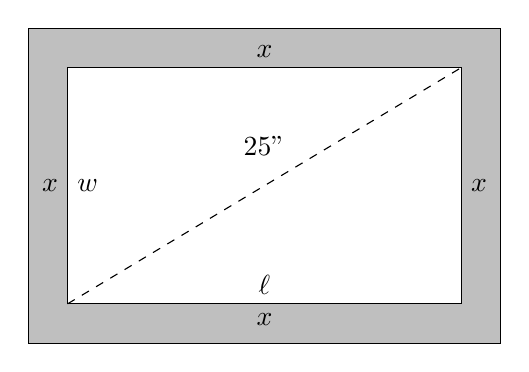
\begin{tikzpicture}
        \draw [fill=lightgray] (-0.5,-0.5) rectangle (5.5,3.5);
        \draw [fill=white] (0,0) rectangle (5,3);
        \draw [dashed] (0,0) -- (5,3);
        \node at (2.5,2.0) {25''};
        \node [above] at (2.5,0) {$\ell$};
        \node [right] at (0,1.5) {$w$};
        \node [above] at (2.5,3) {$x$};
        \node [below] at (2.5,0) {$x$};
        \node [left] at (0,1.5) {$x$};
        \node [right] at (5,1.5) {$x$};
      \end{tikzpicture}
    \end{figure}

    Determine the width of the casing ($x$) around the screen. Round your
    answer to two decimal places.
  \end{enumerate}
\newpage
\item A man stands atop a 256 foot cliff with a ball.
  \begin{enumerate}
  \item How long does it take for the ball to hit the ground if he simply
    releases the ball?

  \item How long does it take for the ball to hit the ground if he throws the
    ball up with a velocity of 16 ft/s? (Hint: keep the negative solution
    around for later).

  \item How long does it take for the ball to hit the ground if he throws the
    ball down with a velocity of 16 ft/s? (Hint: no additional calculations
    are needed).

  \item Assume that a lady is standing on the ground below the cliff and throws
    a ball up so that it passed the man on the cliff at a velocity of 16 ft/s.
    How long would it be before the ball hits the ground? (Hint: you already
    have all the information that you need).
\end{enumerate}

\item For each of the following inequalities, graph the solution set and
  state the solution set in interval notation.
  \begin{enumerate}
  \item $2\abs{5-3x}+7<21$
  \item $2\abs{5-3x}+7\ge21$
  \end{enumerate}

\item Solve for $x$, stating the solution in interval notation.
  \[\frac{x+1}{x-2}<\frac{x-3}{x+4}\]

\item Determine the domain for each of the following expressions, stating each
  in interval notation.
  \begin{enumerate}
    \item \[\sqrt{\frac{x^2-3x-10}{x^2-9x+20}}\]
    \item \[\sqrt[3]{\frac{x^2-3x-10}{x^2-9x+20}}\]
  \end{enumerate}
\end{enumerate}
  
\end{document}
